% !TeX program = xelatex
\documentclass[11pt,fleqn]{article}
\usepackage[letterpaper,margin=0.92in]{geometry}
\usepackage{fontspec}
\setmainfont{Latin Modern Roman}
\setsansfont{Latin Modern Sans}
\setmonofont{Latin Modern Mono}
\usepackage{microtype}
\usepackage{amsmath,amssymb,mathtools,amsthm}
\usepackage{xcolor}
\usepackage{hyperref}
\usepackage{graphicx}
\usepackage{enumitem}
\usepackage{booktabs}
\usepackage{array,tabularx}
\usepackage{listings}
\usepackage{fancyvrb}
\usepackage{fancyhdr}
\usepackage{tikz}
\usepackage{caption}
\captionsetup{font=small,labelfont=bf,labelsep=period}
\hypersetup{colorlinks=true,linkcolor=black,urlcolor=blue!55!black,citecolor=black}
\setlength{\parindent}{1.2em}
\setlength{\parskip}{0pt}
\setlength{\mathindent}{1.7em}
\setlist{nosep,leftmargin=1.6em}
\setlength{\headheight}{14pt}
\pagestyle{fancy}
\fancyhf{}
\fancyhead[L]{\small Ternatrees and A120590}
\fancyhead[R]{\small Bradley Klee}
\fancyfoot[C]{\thepage}
\renewcommand{\headrulewidth}{0.25pt}
\renewcommand{\footrulewidth}{0pt}

\theoremstyle{plain}
\newtheorem*{theorem}{Theorem}
\newtheorem*{lemma}{Lemma}

\definecolor{codegray}{RGB}{95,95,95}
\definecolor{codebg}{RGB}{250,250,250}
\lstdefinestyle{pycode}{
	language=Python,
	basicstyle=\ttfamily\fontsize{7.25}{8.25}\selectfont,
	keywordstyle=\bfseries,
	commentstyle=\color{codegray},
	stringstyle=\itshape,
	showstringspaces=false,
	breaklines=true,
	breakatwhitespace=false,
	columns=fullflexible,
	keepspaces=true,
	frame=tb,
	framerule=0.3pt,
	rulecolor=\color{black!45},
	backgroundcolor=\color{codebg},
	numbers=left,
	numberstyle=\tiny\color{codegray},
	numbersep=5pt,
	xleftmargin=2.1em,
	framexleftmargin=1.8em,
	aboveskip=5pt,
	belowskip=4pt
}

\tikzset{
	ternroot/.style={circle,draw=black,fill=white,inner sep=2.0pt,line width=0.55pt},
	ternleaf/.style={circle,draw=black,fill=black,inner sep=2.0pt,line width=0.55pt},
	ternempty/.style={circle,draw=black,fill=white,inner sep=1.55pt,line width=0.55pt},
	ternedge/.style={draw=black,line width=0.55pt}
}

\newcommand{\poly}[1]{\langle #1\rangle}
\newcommand{\dd}{\,d}

\title{\vspace{-2.1em}\textbf{Ternatrees and OEIS A120590}\\[0.3em]
	\large All the must-have identities, herein derived or re-proven}
\author{Bradley Klee, \quad Mech.An.ika Sol \textnormal{(Open AI)}}
\date{July 30, 2026}

\raggedbottom
\begin{document}
	\maketitle
	
	
	\thispagestyle{empty}
	
	\begin{abstract}
		The sequence $a(n)$ counts rooted ordered ternatrees with $n$ true leaves,
		three ordered child positions, and no unary branching. Each term $a(n)$ can be written as a contour integral 
		for a small loop $\gamma$ around the origin. Summing term integrals gives an 
		integral definition of the ordinary generating function $A(x)$. We can shift 
		one or derive the other to obtain recurrence or differential data directly. 
		This data guarantees the newly revealed geometric model agrees with 
		pre-established conventions from Paul Hanna's extensive investigation 
		almost twenty years ago.  
	\end{abstract}
	
	\begin{theorem}
		The ternatree counting function has many different equivalent definitions,
		and they are all easily certifiable by automated techniques of computer algebra:  
		\begin{enumerate}[label=(\arabic*),leftmargin=2.2em,itemsep=0.55em,topsep=0.35em]
			\item For a sufficiently small closed curve $\gamma$ about the origin,
			\[
			a(0)=1,\qquad
			a(n)=\frac{1}{2\pi i\,n}\oint_\gamma\frac{\dd u}{\rho(u)^n}
			=\frac1n[u^{n-1}]D(u)^{-n}\qquad(n\ge1).
			\]
			where $D(u)=1-3u-u^2$ and $\rho(u)=uD(u)$. 
			
			\item Summing under the integral sign then yields: 
			\[
			A(x)=\sum_{n\geq0}a(n)x^n  = 1-\frac{1}{2\pi i}\oint_\gamma
			\log\!\left(1-\frac{x}{\rho(u)}\right)\dd u.
			\]
			\item Shifting the coefficient definition leads to a p-recurrence:
			\small \[
			-3(3n-1)(3n+1)a(n)-81(n+1)(2n+1)a(n+1)+13(n+1)(n+2)a(n+2)=0.
			\]
			
			\item While deriving the whole-function definition leads to an ODE:
			\[
			(27x^2+162x-13)A''(x)+27(x+3)A'(x)-3A(x)=0.
			\]
			\item Either the p-recurrence or the ODE also determines the original 
			algebraic definition: 
			\[
			4A(x)=3+x+A(x)^3,\qquad A(0)=1.
			\]
			
		\end{enumerate}
		The initial values are
		\[
		1,1,3,19,150,1326,12558,124590,\ldots.
		\]
	\end{theorem}
	
	\clearpage
	\section{Trees, typogeometry, and contour integration}
	
	A \textit{ternatree} is a rooted ordered tree in which every internal vertex 
	has three ordered child positions.  If a vertex does not branch, it is either 
	empty or a true leaf. Unary pass-through is forbidden: if a vertex is branching,
	it must have at least two nonempty children. Here are a few example ternatrees:
	
	\begin{figure}[h]
		\centering
		\begin{minipage}[t]{0.22\textwidth}\centering
			\begin{tikzpicture}[x=1cm,y=1cm,scale=1.0]
				\node[ternleaf] at (0,0.7) {};
			\end{tikzpicture}
			\par\smallskip\(1\)
		\end{minipage}\hfill
		\begin{minipage}[t]{0.22\textwidth}\centering
			\begin{tikzpicture}[x=1cm,y=1cm,scale=1.0]
				\node[ternroot] (r) at (0,1.15) {};
				\node[ternleaf] (a) at (-0.62,0) {};
				\node[ternleaf] (b) at (0,0) {};
				\node[ternempty] (c) at (0.62,0) {};
				\draw[ternedge] (r)--(a) (r)--(b) (r)--(c);
			\end{tikzpicture}
			\par\smallskip\(\{1,1,0\}\)
		\end{minipage}\hfill
		\begin{minipage}[t]{0.22\textwidth}\centering
			\begin{tikzpicture}[x=1cm,y=1cm,scale=1.0]
				\node[ternroot] (r) at (0,1.15) {};
				\node[ternleaf] (a) at (-0.62,0) {};
				\node[ternleaf] (b) at (0,0) {};
				\node[ternleaf] (c) at (0.62,0) {};
				\draw[ternedge] (r)--(a) (r)--(b) (r)--(c);
			\end{tikzpicture}
			\par\smallskip\(\{1,1,1\}\)
		\end{minipage}\hfill
		\begin{minipage}[t]{0.28\textwidth}\centering
			\begin{tikzpicture}[x=1cm,y=1cm,scale=1.0]
				\node[ternroot] (r) at (0,2.0) {};
				\node[ternroot] (a) at (-0.72,1.03) {};
				\node[ternleaf] (b) at (0,1.03) {};
				\node[ternempty] (c) at (0.72,1.03) {};
				\node[ternleaf] (aa) at (-1.15,0) {};
				\node[ternleaf] (ab) at (-0.72,0) {};
				\node[ternempty] (ac) at (-0.29,0) {};
				\draw[ternedge] (r)--(a) (r)--(b) (r)--(c);
				\draw[ternedge] (a)--(aa) (a)--(ab) (a)--(ac);
			\end{tikzpicture}
			\par\smallskip\(\{\{1,1,0\},1,0\}\)
		\end{minipage}
		\caption{A few ternatrees.  Filled endpoints are true leaves, open
			endpoints are empty leaves. Branches are colored as empty for counting 
			purposes. Typogeometric codes are given as labels for each case. }
	\end{figure}
	
	Each ternatree other than the unit conforms to a recursive grammar that 
	produces lists within lists, where each list has length three and the 
	elements are either: another length-3 list, a true leaf, or an empty 
	leaf. A list with two or three empty leaves can never occur. 
	Consider a ternatree with $n$ true leaves, and delete the empty leaves. 
	Assume $i+j$ internal vertices, where the $i$ (or the $j$) branch 
	either by $2$ (or by $3$). Starting from one root we have a constraint: 
	\[
	1+i+2j=n.
	\]
	where the multipliers $1=2-1$ and $2=3-1$ subtract out a constant $1$ 
	to account for motion through intermediary nodes. 
	
	The entire tree has $z=n+i+j$ vertices.  Write $\Delta_2=+1$ 
	for a two-child vertex, $\Delta_3=+2$ for a three-child vertex, 
	and $l=-1$ for a true leaf. A valid $\{\Delta_x,l\}$-word must
	have letters summing to $-1$. The cycle lemma~[6,7] says that exactly one cyclic shift is valid. 
	
	Let $\mathcal{W}_z$ be a word of length $z$ over $\{\Delta_2,\Delta_3,l\}$. 
	When reading left to right, letters gather into trees by opening $x$ branches 
	at each $\Delta_x$ and by filling open branches with subtrees and true leaves 
	consecutively as they open. Assume that subtrees inherit priority so that the 
	word $\mathcal{W}_z$ follows from depth-first scan. A valid word cannot start 
	with $l$, because we need a $\Delta_2$ or $\Delta_3$ to open branch vacancies 
	first. A valid word must start with $\Delta_2$ or $\Delta_3$. Conversely, 
	when reading right to left, a valid word must start with at least two or 
	three true leaves. In general, the deepest complete subtree $t_r$ is found after 
	arbitrarily many end leaves by backtracking left to right from the rightmost 
	branching letter. 
	
	\begin{lemma}
		The set of $z$ cyclic shifts of $\mathcal{W}_z$, denoted
		$\langle \mathcal{W}_z \rangle$, contains a unique valid element
		$\mathcal{W}_z'$ whose initial letter is either $\Delta_2$ or $\Delta_3$.
	\end{lemma}
	
	
	\begin{proof}	
		Consider the set $\langle \mathcal{W}_z \rangle$ as the letters 
		of $\mathcal{W}_z$ written around the circumference of a circle. Regard 
		each true leaf $l$ as a complete subtree $t$. A deconstruction step replaces
		either $\Delta_2+t+t$ or $\Delta_3+t+t+t$ by a single complete subtree $t$. 
		For a valid word, reading a depth-first scan in reverse gives one possible 
		order of deconstruction. 
		
		After any number of deconstruction steps, let $N$ be the 
		number of complete subtree blocks, and let $I$ and $J$ be the numbers 
		of unresolved letters $\Delta_2$ and $\Delta_3$. Every complete subtree 
		inherits total weight $-1$, so conservation of total weight gives 
		$1+I+2J=N$, as before, at any partial deconstruction.
		
		Suppose that unresolved branching letters remain but no deconstruction
		step is possible. Then each unresolved $\Delta_2$ is followed, before
		the next unresolved branching letter, by at most one complete subtree,
		and each unresolved $\Delta_3$ is followed by at most two. These runs
		contain all $N$ complete subtrees, so $N\leq I+2J$, contradicting
		$N=1+I+2J$. Hence a deconstruction step is always possible until every
		branching letter has been resolved. When $I=J=0$, the same identity
		gives $N=1$, so the entire circular word has become one complete tree.
		
		The final root is independent of the order of deconstruction. Indeed,
		two steps available at the same stage are disjoint: each consists of
		one unresolved branching letter followed by its required consecutive
		complete subtrees. They may therefore be performed in either order or
		in parallel, with the same result. The deconstruction 
		process must reach a fixed point where $I+J=0$ and $N=1$. The first 
		symbol of the final complete subtree is either $\Delta_2$ or $\Delta_3$. 
		Reading the circular word left to right from this unique root 
		returns the unique $\mathcal{W}_z'$.
	\end{proof}
	
	As an immediate corollary to the cycle lemma, we can count the number of 
	distinct words $\mathcal{W}_z$ per $z$ and by letter distributions as: 
	\[
	\frac{1}{z}\binom{z}{n,i,j}.
	\]
	A factor $3^i$ later appears in the numerator to account for re-insertion 
	of empty nodes to $\Delta_2$ subtrees. Using our earlier constraints,
	\[
	i=n-1-2j,
	\qquad
	z=2n-1-j,
	\]
	we can then sum over letter distributions to obtain the $a(n)$ counts of 
	trees or typogeometries per true leaf count $n$:
	\[
	a(n) =
	\sum_{j=0}^{\lfloor(n-1)/2\rfloor}
	3^{n-1-2j} \frac{1}{2n-1-j}
	\binom{2n-1-j}{n,\;n-1-2j,\;j}.
	\]
	\[
	a(n) =
	\sum_{j=0}^{\lfloor(n-1)/2\rfloor}
	3^{n-1-2j}\frac{(2n-2-j)!}
	{n!\,(n-1-2j)!\,j!}.
	\]
	\[
	a(n)=\frac1n\sum_{j=0}^{\lfloor(n-1)/2\rfloor}
	3^{n-1-2j}
	\binom{2n-2-j}{n-1}
	\binom{n-1-j}{j}.
	\]
	The sum in the final expression is precisely the coefficient of
	$u^{n-1}$ in $(1-3u-u^2)^{-n}$. First apply the negative-binomial
	expansion with $x=3u+u^2$:
	\[
	(1-3u-u^2)^{-n}
	=
	\sum_{k\geq 0}
	\binom{n+k-1}{k}(3u+u^2)^k.
	\]
	Then apply the ordinary binomial theorem to the remaining terms:
	\[
	(1-3u-u^2)^{-n}
	=
	\sum_{k\geq 0}\sum_{j=0}^{k}
	\binom{n+k-1}{k}
	\binom{k}{j}
	3^{k-j}u^{k+j}.
	\]
	Selecting the terms with $k+j=n-1$, and hence setting
	$k=n-1-j$, yields:
	\[
	[u^{n-1}](1-3u-u^2)^{-n}
	=
	\sum_{j=0}^{\lfloor(n-1)/2\rfloor}
	3^{n-1-2j}
	\binom{2n-2-j}{n-1}
	\binom{n-1-j}{j}.
	\]
	Thus, with $D(u)=1-3u-u^2$ we obtain
	\[
	a(n)=\frac1n[u^{n-1}]D(u)^{-n}.
	\]
	
	Cauchy's coefficient formula gives the integral form:
	\[
	a(n)=\frac{1}{2\pi i\,n}\oint_\gamma
	\frac{\dd u}{u^nD(u)^n}
	=\frac{1}{2\pi i\,n}\oint_\gamma\frac{\dd u}{\rho(u)^n},
	\]
	where $\gamma$ is a small contour around the pole at the origin. 
	Summing terms over the small disk, we obtain a generating function:
	\[
	\begin{aligned}
		A(x)
		&=1+\sum_{n\ge1}\frac{x^n}{2\pi i\,n}
		\oint_\gamma\frac{\dd u}{\rho(u)^n}\\
		&=1+\frac{1}{2\pi i}\oint_\gamma
		\sum_{n\ge1}\frac1n\left(\frac{x}{\rho(u)}\right)^n\dd u\\
		&=1-\frac{1}{2\pi i}\oint_\gamma
		\log\!\left(1-\frac{x}{\rho(u)}\right)\dd u.
	\end{aligned}
	\]
	This is the integral definition of the ordinary generating function near the
	origin.
	
	\section{Shift reduction and the recurrence}
	
	We now work backward from known certificate data for the integrands
	\[
	H_n(u)=\frac{1}{n\rho(u)^n},
	\qquad n\geq1,
	\]
	and reconstruct the reduction that produces the recurrence; compare~[2--5,10].
	
	For $w=(w_0,w_1,w_2)^T$, put
	$\poly{w}=w_0+w_1u+w_2u^2$. The fixed reduction operators are
	\[
	U=\frac1{13}
	\begin{pmatrix}
		153&24&3\\72&9&6\\0&0&0
	\end{pmatrix},\qquad
	V=\frac1{13}
	\begin{pmatrix}
		-13&0&0\\75&11&3\\24&3&2
	\end{pmatrix},\qquad
	J=\begin{pmatrix}0&1&0\\0&0&2\\0&0&0\end{pmatrix}.
	\]
	They satisfy
	\[
	\rho\poly{Uw}-\rho'\poly{Vw}=\poly{w},
	\qquad
	\poly{Jw}=\frac{d}{du}\poly{w}.
	\]
	Hence, for $m\geq1$,
	\[
	\frac{\poly{w}}{\rho^{m+1}}
	=
	\frac{\poly{(U-JV/m)w}}{\rho^m}
	+\frac{d}{du}\left(\frac{\poly{Vw}}{m\rho^m}\right).
	\]
	The integral of the last term around $\gamma$ is zero, so each
	application removes one power of $\rho$ while retaining the numerator
	in the same three-dimensional space. Define
	\[
	\operatorname{Lower}(w,m)
	=
	\left(U-\frac1mJV\right)w.
	\]
	
	With $e=(1,0,0)^T$, define
	\[
	c_0=e,\qquad
	c_1=\frac{n}{n+1}\operatorname{Lower}(e,n),\qquad
	c_2=\frac{n}{n+2}\operatorname{Lower}
	\bigl(\operatorname{Lower}(e,n+1),n\bigr).
	\]
	These are the numerator vectors obtained by reducing
	$H_n,H_{n+1},H_{n+2}$ to the common denominator $\rho^n$, apart from
	the common factor $1/n$.
	
	Arrange the three vectors as the columns of
	\[
	X(n)=
	\begin{pmatrix}
		c_0&c_1&c_2
	\end{pmatrix}
	=
	\begin{pmatrix}
		1&
		\dfrac{3(51n-25)}{13(n+1)}&
		\dfrac{3(8379n^2+81n-2038)}
		{169(n+1)(n+2)}
		\\[6pt]
		0&
		\dfrac{24(3n-2)}{13(n+1)}&
		\dfrac{1944(2n+1)(3n-2)}
		{169(n+1)(n+2)}
		\\[6pt]
		0&0&0
	\end{pmatrix}.
	\]
	We find coefficients $P_0(n),P_1(n),P_2(n)$ in the nullspace of $X(n)$:
	\[
	X(n)
	\begin{pmatrix}
		P_0(n)\\P_1(n)\\P_2(n)
	\end{pmatrix}
	=0 \implies
	\begin{pmatrix}
		P_0(n)\\P_1(n)\\P_2(n)
	\end{pmatrix}
	=
	\begin{pmatrix}
		-3(3n-1)(3n+1)\\
		-81(n+1)(2n+1)\\
		13(n+1)(n+2)
	\end{pmatrix}.
	\]
	Because each lowering step differs from its reduced representative by
	an exact derivative, the vector relation lifts to the exact identity
	\[
	P_0H_n+P_1H_{n+1}+P_2H_{n+2}
	=
	\frac{d}{du}\bigl(R(n,u)H_n(u)\bigr),
	\]
	where
	\[
	R(n,u)=
	\frac{-9nu^4-36nu^3+6nu^2+84nu-13n
		-3u^4-12u^3-6u^2+3u}{\rho(u)}.
	\]
	Integrating around $\gamma$ eliminates the exact derivative and gives
	\[
	P_0(n)a(n)+P_1(n)a(n+1)+P_2(n)a(n+2)=0.
	\]
	
	Before moving on, we show how the reduction operators $U$ and $V$ arise from a
	single coefficient matrix. The matrix $G$ represents the coefficient map
	$(a,b)\mapsto\rho a-\rho'b$ in the bases $1,u,u^2$ for $a,b$ and
	$1,u,\ldots,u^5$ for the result:
	\[
	G=
	\begin{pmatrix}
		0&0&0&-1&0&0\\
		1&0&0&6&-1&0\\
		-3&1&0&3&6&-1\\
		-1&-3&1&0&3&6\\
		0&-1&-3&0&0&3\\
		0&0&-1&0&0&0
	\end{pmatrix}.
	\]
	Let
	\[
	E=\begin{pmatrix}I_3\\0\end{pmatrix}.
	\]
	Since $\det G=-13$, the matrix is invertible, and
	\[
	\begin{pmatrix}
		U\\V
	\end{pmatrix}
	=G^{-1}E.
	\]
	The derivative matrix $J$ enters in the next step
	through $\poly{Vw}'=\poly{JVw}$.
	
	\clearpage
	\section{Derivative reduction and the ODE}
	
	\begin{center}
		\renewcommand{\arraystretch}{1.22}
		\begin{tabularx}{\textwidth}{>{\raggedright\arraybackslash}p{0.20\textwidth}
				>{\raggedright\arraybackslash}X
				>{\raggedright\arraybackslash}X}
			\toprule
			& \textbf{Shift in $n$} & \textbf{Derivative in $x$}\\
			\midrule
			Integral family
			& $H_{n+r}(u)=1/((n+r)\rho(u)^{n+r})$
			& $\partial_x^r\Phi(x,u)=r!\Phi(x,u)^{r+1}$\\
			Denominator
			& $\rho(u)$
			& $\Phi(x,u)^{-1}=\rho(u)-x$\\
			Coefficient map
			& $G$
			& $G_x=G-xEE^T$\\
			Inverse blocks
			& $U,V$ over $\mathbb Q$
			& $U_x,V_x$ over $\mathbb Q(x)$\\
			Reduced columns
			& $H_n,H_{n+1},H_{n+2}$
			& $\Phi,\partial_x \Phi,\partial_x^2 \Phi$\\
			Kernel
			& $(P_0(n),P_1(n),P_2(n))^T$
			& $(24,81x+243,\det G_x)^T$\\
			Consequence
			& recurrence for $a(n)$
			& differential equation for $A(x)$\\
			\bottomrule
		\end{tabularx}
	\end{center}
	
	The construction from the preceding section extends to derivatives
	of the generating function by differentiation under the integral sign. We begin
	with the rational first derivative: 
	\[
	A'(x)=\frac{1}{2\pi i}\oint_\gamma \Phi(x,u)\dd u,
	\qquad \text{where} \qquad 
	\Phi(x,u)=\frac1{\rho(u)-x}.
	\]
	The corresponding matrix data is: 
	\[
	G_x=
	\begin{pmatrix}
		-x&0&0&-1&0&0\\
		1&-x&0&6&-1&0\\
		-3&1&-x&3&6&-1\\
		-1&-3&1&0&3&6\\
		0&-1&-3&0&0&3\\
		0&0&-1&0&0&0
	\end{pmatrix},
	\qquad
	G_x^{-1}E=\binom{U_x}{V_x},
	\qquad
	\Delta(x)=\det G_x=27x^2+162x-13.
	\]
	Notice that $G_0=G$. The matrix is also invertible near the origin, so we obtain:  
	\[
	\!\! U_x=\frac1{\Delta(x)}
	\begin{pmatrix}
		-27x-153&-24&-9x-3\\
		-72&-27x-9&54x-6\\
		0&0&0
	\end{pmatrix},
	\;
	V_x=\frac1{\Delta(x)}
	\begin{pmatrix}
		13-9x&24x&9x^2+3x\\
		-9x-75&-9x-11&15x-3\\
		-24&-9x-3&18x-2
	\end{pmatrix},
	\]
	and with $J_x=J$, define
	\[
	\operatorname{Lower}_x(w,m)
	=
	\left(U_x-\frac1mJ_xV_x\right)w.
	\]
	The integrands $\Phi$, $\partial_x\Phi$, and $\partial_x^2\Phi$ have
	pole orders $1$, $2$, and $3$, respectively. Reducing them to the common
	denominator $\rho(u)-x$ gives the basis vectors 
	\[
	d_0=e,
	\qquad
	d_1=\operatorname{Lower}_x(e,1),
	\qquad
	d_2=
	2\operatorname{Lower}_x
	\bigl(\operatorname{Lower}_x(e,2),1\bigr).
	\]
	Arranging the reduced numerator vectors as the columns of
	\[
	X_x=
	\begin{pmatrix}
		d_0&d_1&d_2
	\end{pmatrix}
	= \begin{pmatrix}
		1&
		-\dfrac{6(3x+13)}{\Delta}&
		\dfrac{6(135x^2+1134x+3211)}{\Delta^2}
		\\[7pt]
		0&
		-\dfrac{24}{\Delta}&
		\dfrac{1944(x+3)}{\Delta^2}
		\\[7pt]
		0&0&0
	\end{pmatrix},
	\]
	and its null space is identified by
	\[
	X_x
	\begin{pmatrix}
		24\\
		81x+243\\
		\Delta(x)
	\end{pmatrix}
	=0.
	\]
	Consequently, the corresponding combination of the original integrands
	is an exact derivative:
	\[
	24\Phi+(81x+243)\partial_x\Phi
	+\Delta(x)\partial_x^2\Phi
	=
	\frac{d}{du}
	\left(
	N(x,u)\Phi^2
	\right),
	\]
	where $N(x,u)=12u^4+48u^3+3ux-87u+3x+13.$ Since $u$-integration around $\gamma$ 
	eliminates the exact derivative, we next obtain:
	\[
	\Delta(x)A'''(x)
	+(81x+243)A''(x)
	+24A'(x)=0.
	\]
	This is the derivative of
	\[
	\Delta(x)A''(x)
	+27(x+3)A'(x)
	-3A(x)=C.
	\]
	Finally, $A(0)=1, \; A'(0)=1, \; A''(0)=6$ determine $C=0$. Therefore
	\[
	(27x^2+162x-13)A''(x)
	+27(x+3)A'(x)
	-3A(x)=0.
	\]
	
	
	
	\medskip
	
	Now we can use the ODE to prove the algebraic generating function. Let
	$\widetilde A(x)$ be the branch of
	\[
	F(x,\widetilde A)=\widetilde A^3-4\widetilde A+x+3=0
	\]
	satisfying $\widetilde A(0)=1$. Implicit differentiation gives
	\[
	\widetilde A'=\frac{1}{4-3\widetilde A^2},
	\qquad
	\widetilde A''=\frac{6\widetilde A}{(4-3\widetilde A^2)^3}.
	\]
	Substitution into the differential equation and clearing denominators yields
	\[
	\begin{aligned}
		&(4-3\widetilde A^2)^3
		\left(
		(27x^2+162x-13)\widetilde A''
		+27(x+3)\widetilde A'
		-3\widetilde A
		\right)\\
		&\qquad=
		27\bigl(\widetilde A^3-4\widetilde A+x+3\bigr)
		\bigl(3\widetilde A^4+6\widetilde A x
		+18\widetilde A+16\bigr).
	\end{aligned}
	\]
	The right-hand side vanishes modulo $F(x,\widetilde A)$, so
	$\widetilde A$ satisfies the ODE. Moreover,
	\[
	\widetilde A(0)=1,
	\qquad
	\widetilde A'(0)=1.
	\]
	Since the leading coefficient of the ODE is nonzero at the origin, the
	solution with these initial values is unique there. Therefore
	$\widetilde A(x)=A(x)$, and
	\[
	A^3-4A+x+3=0.
	\]  
	
	
	\clearpage
\section{Relations among the formulas}

The geometric count, integral definition, recurrence, differential equation,
and algebraic equation determine the same series. Their relations are
\[
\begin{array}{l}
    \text{ternatree profiles}
    \longrightarrow
    \displaystyle a(n)=\frac{1}{2\pi i\,n}
    \oint_\gamma\frac{\dd u}{\rho(u)^n},\\[1.1em]
    \text{shift the integrand's exponent}
    \longrightarrow
    \text{P-recurrence},\\[0.6em]
    \text{summation under the integral}
    \longrightarrow
    \displaystyle A(x)=1-\frac{1}{2\pi i}\oint_\gamma
    \log\!\left(1-\frac{x}{\rho(u)}\right)\dd u,\\[0.6em]
    \text{differentiate and reduce under the integral}
    \longrightarrow
    \text{ODE},\\[0.6em]
    \text{P-recurrence}
    \longleftrightarrow
    \text{ODE},\\[0.6em]
    F(x,A)=A^3-4A+x+3
    \longrightarrow
    \text{implicit differentiation and substitution into the ODE},\\[0.6em]
    A(0)=1,\quad A'(0)=1
    \longrightarrow
    \text{uniqueness of the ODE solution}
    \longrightarrow
    4A=3+x+A^3.
\end{array}
\]
The recurrence and differential equation correspond coefficient by
coefficient. The algebraic form is verified as an ansatz: its branch through
$A(0)=1$ satisfies the same ODE and initial values, and therefore coincides
with the generating function.

\clearpage
	\section{Reference pseudocode}
	
	The following specification implements the shift reduction.  It constructs the
	remainder matrix, extracts its primitive kernel vector, verifies the certificate,
	generates the sequence, and converts the recurrence into the differential equation.
	\begin{center}
	\begin{minipage}{0.96\textwidth}
	\VerbatimInput[fontsize=\fontsize{7.4}{8.4}\selectfont,frame=lines]
	{.support/source/ternatree_one_page_crank_academic.txt}
	\end{minipage}
	\end{center}
	
	\clearpage
	\section{Pseudocode operations and exact realization}
	\begin{figure}[h]
		\centering
		\begin{minipage}[t]{0.485\textwidth}
		\centering
		\textbf{(a) Pseudocode}\par\smallskip
		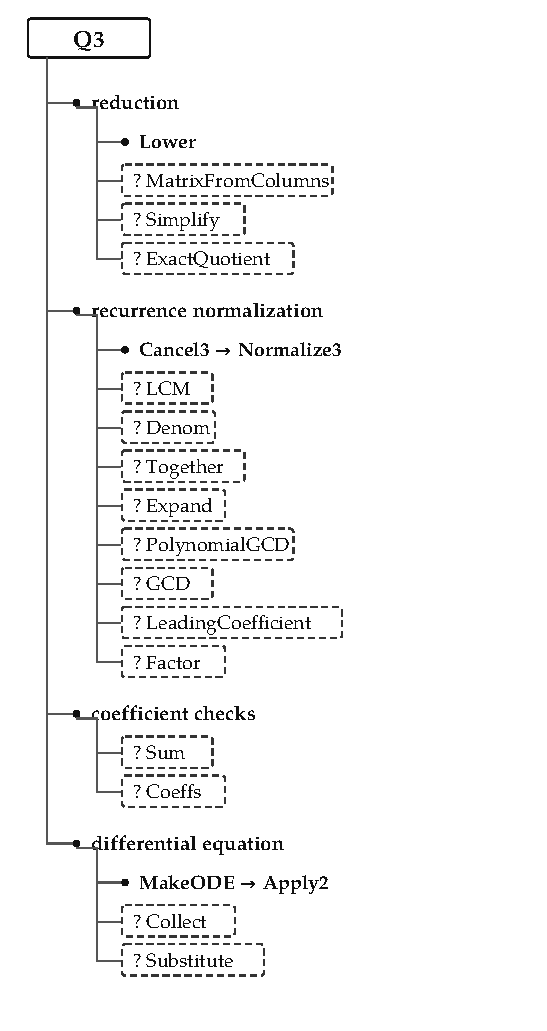
\includegraphics[width=\linewidth,height=0.72\textheight,keepaspectratio]
		{.support/graphs/ternatree_pseudocode_mysteries.pdf}
		\end{minipage}\hfill
		\begin{minipage}[t]{0.485\textwidth}
		\centering
		\textbf{(b) SymPy implementation}\par\smallskip
		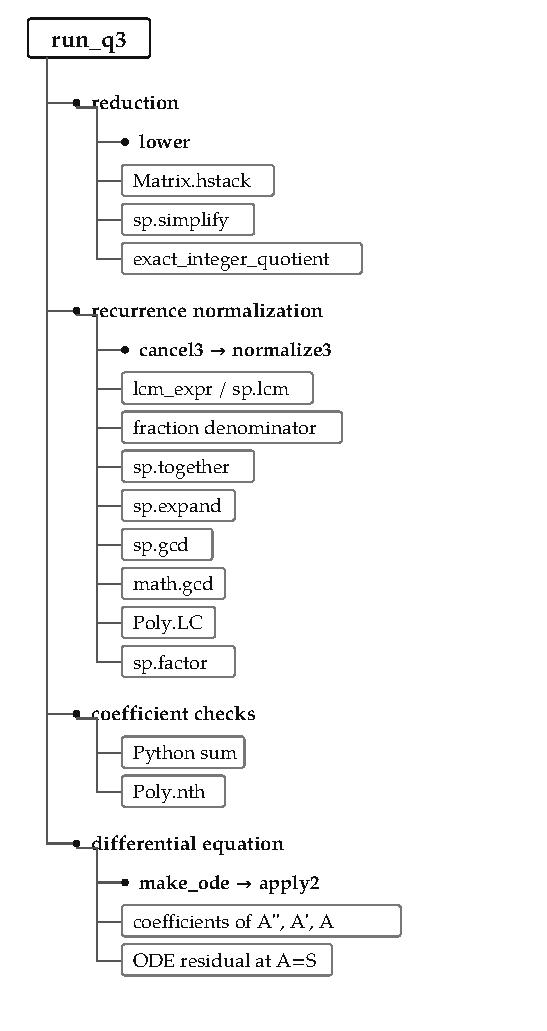
\includegraphics[width=\linewidth,height=0.72\textheight,keepaspectratio]
		{.support/graphs/ternatree_sympy_resolutions.pdf}
		\end{minipage}
		\caption{The local routines and their algebraic dependencies.  Dashed leaves
			are operations used but not defined in the pseudocode; the corresponding rows
			on the right identify their exact realization.}
	\end{figure}
	
	\clearpage
\section{References by method}

The references are ordered by the methods actually used in the calculation.
Basic complex calculus and coefficient extraction come first; the more
specialized combinatorial and symbolic-computation references follow.
\begin{sloppypar}
\begin{enumerate}[label={[\arabic*]},leftmargin=2.4em,itemsep=0.52em]
\item \textbf{Lars V. Ahlfors}, \emph{Complex Analysis: An Introduction to
the Theory of Analytic Functions of One Complex Variable}, third edition,
McGraw--Hill, 1979. Standard background for power series, complex integration,
Cauchy's formula, and differentiation of contour integrals.

\item \textbf{Peter Henrici}, \emph{Applied and Computational Complex
Analysis}, Volume 1: \emph{Power Series--Integration--Conformal
Mapping--Location of Zeros}, Wiley, 1974; Wiley Classics Library reprint,
1988. A calculus-oriented reference for formal and analytic power series,
complex integration, partial fractions, and exact coefficient extraction.

\item \textbf{Ira M. Gessel}, ``Lagrange inversion,'' \emph{Journal of
Combinatorial Theory, Series A} \textbf{144} (2016), 212--249. DOI:
\nolinkurl{10.1016/j.jcta.2016.06.018}. A focused survey of the inversion
formula used to extract the coefficients from the implicit equation.

\item \textbf{Richard P. Stanley}, \emph{Enumerative Combinatorics},
Volume 2, second edition, Cambridge University Press, 2023. Chapters 5--6
cover trees, composition and inversion of generating functions, and algebraic
and D-finite series.

\item \textbf{Philippe Flajolet and Robert Sedgewick}, \emph{Analytic
Combinatorics}, Cambridge University Press, 2009. General background for
recursive tree specifications, ordinary generating functions, coefficient
extraction, and the complex-analytic viewpoint.

\item \textbf{Aryeh Dvoretzky and Theodore Motzkin}, ``A problem of
arrangements,'' \emph{Duke Mathematical Journal} \textbf{14} (1947),
305--313. The cycle-lemma source used for the circular-word count.

\item \textbf{George N. Raney}, ``Functional composition patterns and power
series reversion,'' \emph{Transactions of the American Mathematical Society}
\textbf{94} (1960), 441--451. DOI:
\nolinkurl{10.1090/S0002-9947-1960-0114765-9}. Relates prefix words, rooted
trees, functional composition, and power-series reversion.

\item \textbf{Alin Bostan, Shaoshi Chen, Fr\'ed\'eric Chyzak, Ziming Li,
and Guoce Xin}, ``Hermite reduction and creative telescoping for
hyperexponential functions,'' in \emph{ISSAC 2013}, 77--84. DOI:
\nolinkurl{10.1145/2465506.2465946}. Relevant to reduction modulo exact
derivatives and the construction of compact rational certificates.

\item \textbf{Fr\'ed\'eric Chyzak}, ``An extension of Zeilberger's fast
algorithm to general holonomic functions,'' \emph{Discrete Mathematics}
\textbf{217} (2000), 115--134. DOI:
\nolinkurl{10.1016/S0012-365X(99)00259-9}. General background for certified
recurrence and differential reductions.

\item \textbf{OEIS Foundation Inc.}, ``A120590,'' entry initiated by
Paul D. Hanna (2006). The target record and its currently cataloged formulas,
recurrences, and cross-references.
\href{https://oeis.org/A120590}{oeis.org/A120590}.
\end{enumerate}
\end{sloppypar}

	\appendix
	\section{Exact SymPy implementation}
	
	This implementation merges one-shot code produced independently by Kimi (Moonshot AI) and Claude (Anthropic AI), both working from the pseudocode and implementation presented in Sections 5--6.
	
	\subsection{Arithmetic and one-step lowering}
	The functions below define exact least common multiples and the map
	$w\mapsto (U-JV/m)w$.
	\par\medskip\noindent
	\begin{minipage}[t]{\textwidth}
	\lstinputlisting[style=pycode,firstline=1,lastline=24,firstnumber=1]
	{ternatree_q3.py}
	\end{minipage}
	
	\clearpage
	\subsection{Primitive recurrence normalization}
	This function clears rational denominators, removes common polynomial and
	integer factors, and fixes the sign of the recurrence vector.
	\par\medskip\noindent
	\begin{minipage}[t]{\textwidth}
	\lstinputlisting[style=pycode,firstline=26,lastline=58,firstnumber=26]
	{ternatree_q3.py}
	\end{minipage}
	
	\clearpage
	\subsection{Kernel vector and recurrence-to-ODE map}
	The $2\times3$ minors form the kernel vector.  The remaining functions convert
	quadratic recurrence coefficients into the coefficients of $A''$, $A'$, and
	$A$.
	\par\medskip\noindent
	\begin{minipage}[t]{\textwidth}
	\lstinputlisting[style=pycode,firstline=61,lastline=99,firstnumber=61]
	{ternatree_q3.py}
	\end{minipage}
	
	\clearpage
	\subsection{Certificate and term generation}
	The driver constructs $X$, derives the recurrence, verifies the exact
	certificate identity, and generates terms by exact division.
	\par\medskip\noindent
	\begin{minipage}[t]{\textwidth}
	\lstinputlisting[style=pycode,basicstyle=\ttfamily\fontsize{6.65}{7.45}\selectfont,
	 firstline=102,lastline=160,firstnumber=102]
	{ternatree_q3.py}
	\end{minipage}

	\clearpage
	\subsection{Series checks and command-line output}
	The remaining code checks the algebraic and differential equations and
	prints the certificate, recurrence, ODE, and requested terms.
	\par\medskip\noindent
	\begin{minipage}[t]{\textwidth}
	\lstinputlisting[style=pycode,basicstyle=\ttfamily\fontsize{6.65}{7.45}\selectfont,
	 firstline=162,lastline=228,firstnumber=162]
	{ternatree_q3.py}
	\end{minipage}
	
\end{document}
